\chapter{Mt. Gagazet}
\begin{enumerate}
	\item Walk up, \cs[3:40], walk up, \sd
\end{enumerate}
\begin{battle}{Biran and Yenke}
	\begin{itemize}
		\kimahrif Steal from Biran
		\kimahrif Gem Yenke
		\kimahrif Gem Biran
	\end{itemize}
	Pay attention to your drops, they affect \yuna's sphere grid below.
\end{battle}
\end{multicols}
\begin{spheregrid}
	\begin{multicols}{2}
		\begin{itemize}
			\luluf
			\begin{itemize}
				\item Move $\uparrow\uparrow$
				\item Level 2 Key Sphere
				\item Move $\downarrow x9$
				\item Level 3 Key Sphere
				\item Move $\searrow\searrow$
			\end{itemize}
			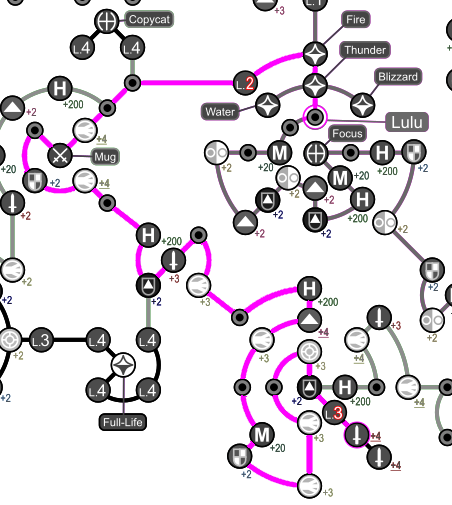
\includegraphics[width=.75\columnwidth]{graphics/lulu_grid}
			\yunaf
			\begin{itemize}
				\item \textit{If you got \textbf{4 Return Spheres}:}
				      \begin{itemize}
					      \item Return to the last Str+2 node in \wakka's grid, Hold $\searrow$
					      \item Move $\leftarrow$
					      \item Mag+3, Level 1 Key Sphere
					      \item Move $\downarrow\downarrow$
					      \item Str+2, Agi+4
				      \end{itemize}
				      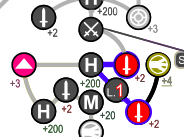
\includegraphics[width=.5\columnwidth]{graphics/4_returns_1}
				\item \textit{If you got \textbf{2 Return Spheres}:}
				      \begin{itemize}
					      \item Friend Sphere to \lulu,  $\downarrow\downarrow$
					      \item Str+4, Str+4
					            \luluf Move $\nearrow\uparrow\uparrow$
					            \yunaf Friend Sphere to \lulu,
					      \item Str+3, Agi+4, Agi+4
				      \end{itemize}
				      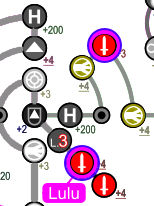
\includegraphics[width=.4\columnwidth]{graphics/2_and_2}
				      \columnbreak
				\item \textit{If you got \textbf{0 Return Spheres}:}
				      \begin{itemize}
					      \tidusf Move to Str+4 by Mental Break $\rightarrow x3, \downarrow, \rightarrow x3$
					      \yunaf Friend Sphere to \tidus
					      \item Str+4
					            \tidusf Move $\nwarrow\leftarrow$ or $\swarrow\swarrow$
					      \item Armor Break
					      \item Do the 2 Return Sphere Menu
					            \rikkuf: Move $\downarrow x5$
					            \yunaf Friend to \rikku\ $\downarrow$
					      \item Agi+4, MgDef +2
					      \item Move $\leftarrow$
					      \item Str+2
				      \end{itemize}
				      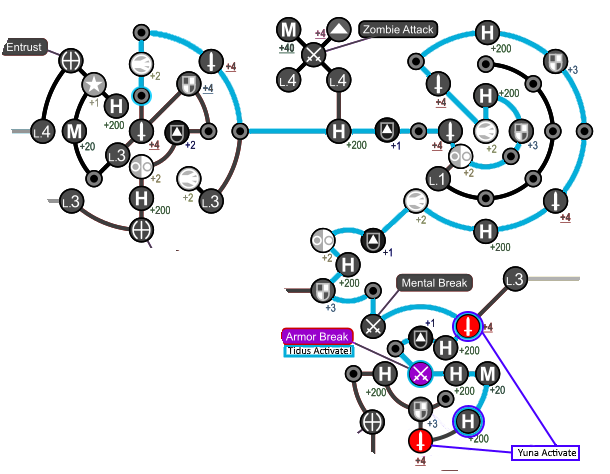
\includegraphics[width=.9\columnwidth]{graphics/post_BY_0_returns}
				      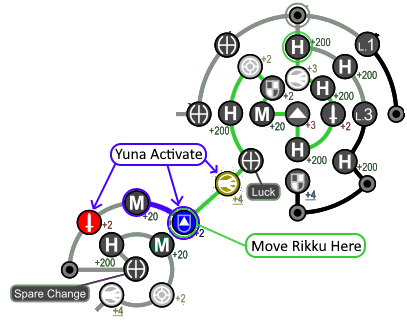
\includegraphics[width=.7\columnwidth]{graphics/0_returns_pt2}
			\end{itemize}
			\item \tidus\ \textit{if you didn't get Armor Break:}
			      \begin{itemize}
				      \item \textit{If you got \textbf{4 Return Spheres}:}
				            \begin{itemize}
					            \item Return Sphere $\downarrow\searrow\searrow$, Str+4 near Armor Break
					            \item Move $\nwarrow\leftarrow$ or $\swarrow\swarrow$
				            \end{itemize}
				      \item \textit{If you got \textbf{2 Return Spheres}:}
				            \begin{itemize}
					            \item Move to Armor Break $\rightarrow x3, \downarrow x6$
				            \end{itemize}
				      \item Armor Break
			      \end{itemize}

		\end{itemize}
	\end{multicols}
\end{spheregrid}
\begin{multicols}{2}
\begin{enumerate}[resume]
	\item \textit{If you had 2 or 4 \textbf{Return Spheres}:}
	      \begin{itemize}
		      \item Customize:
		            \begin{itemize}
			            \auronf Shimmering Blade $\rightarrow$ First Strike
			            \yunaf Staff $\rightarrow$ First Strike
		            \end{itemize}
	      \end{itemize}
	\item \formation{\tidus}{\rikku}{\auron} \textit{If you need need to build up \rikku\ \od\ else } \formation{\tidus}{\kimahri}{\wakka}.
\end{enumerate}

\begin{equip}
	\begin{itemize}
		\auronf Sonic Blade
	\end{itemize}
\end{equip}
\begin{enumerate}[resume]
	\item Walk up, \sd, \cs[1:20], continue walking up, avoid the gravestones.
	\item Make sure you charge \rikku's \od, can skip if you still have a Silence Grenade, by taking the small robot fights, stealing from the small robot, and running with the other characters.
	\item Follow the path around.
	\item Once you're on the Seymour Flux screen, if you're using \rikku\ \od, then Hi-Potion Rikku
	\item \formation{\tidus}{\yuna}{\auron} \textit{If you had 2 or 4 Return Spheres else } \formation{\tidus}{\kimahri}{\wakka}
\end{enumerate}
\begin{battle}[70000]{Seymour Flux}
	\begin{itemize}
		\item \textit{If you had 2 or 4 \textbf{Return Spheres}:}
		      \begin{itemize}
			      \yunaf Attack
			      \tidusf Haste \yuna
			      \switch{\auron}{\rikku}
			      \rikkuf Silence Grenade or \od\ HP Sphere + Grenade
			      \summon{\bahamut}
			      \bahamutf Impulse
			      \yunaf Attack
			      \tidusf Attack. If \yuna\ crit, skip the second Attack to try and get Overkill
		      \end{itemize}
		\item \textit{If you had 0 \textbf{Return Spheres}:}
		      \begin{itemize}
			      \switch{\tidus}{\yuna}
			      \summon{\bahamut}
			      \bahamutf Attack
		      \end{itemize}
	\end{itemize}
\end{battle}
\begin{enumerate}[resume]
	\item \formation{\tidus}{\kimahri}{\auron}
	\item \save\ if \bahamut was banished, Walk to the next screen. \skippablefmv[0:20], \sd, walk up to \tidus\ House, go into the center, \sd. Follow the boy outside, speak to him upstairs, \sd.
	\item Walk up to the next screen, go up the steps. Go down the left path into the water, \sd, swim up. Go up the steps, play the minigame, return to the previous screen.
	\item \tidus\ can attack Splashers for Power Spheres if needed. Try to only attack the 3 fish groups.
	\item Return to Save Sphere, go up and left, then go down the right path, swim up into the next screen. Complete the minigame, \rikku\ Green, \tidus\ Blue, \wakka\ Red. Return.
	\item Go up left path, \sd, continue up the path, \save\ if \bahamut\ was banished and you didn't touch one earlier.
	\item \formation{\tidus}{\yuna}{\kimahri}. Go onto the next screen.
\end{enumerate}
\begin{battle}[40000]{Sanctuary Keeper}
	\begin{itemize}
		\item \textit{If 2 or 4 \textbf{Return Spheres}:}
		      \begin{itemize}
			      \yunaf Defend
			      \tidusf Armor Break
		      \end{itemize}
		\item \textit{If 0 \textbf{Returns Spheres}:}
		      \begin{itemize}
			      \tidusf Defend
		      \end{itemize}
		      \summon{\bahamut}
		      \bahamutf Attack
	\end{itemize}
\end{battle}